\documentclass[runningheads]{llncs}

% Khai báo các gói thư viện cần thiết
\usepackage[utf8]{inputenc}
\usepackage[T5]{fontenc} 
\usepackage[english]{babel} % Đổi sang tiếng Anh để Overleaf ngắt dòng chuẩn
\usepackage{cite}
\usepackage{amsmath,amssymb,amsfonts}
\usepackage{graphicx}
\usepackage{textcomp}
\usepackage{xcolor}
\usepackage{booktabs}
\usepackage{calc}
\usepackage{url}
\usepackage{hyperref}
\begin{document}

% --- TIÊU ĐỀ BÀI BÁO (Springer LNCS Style) ---
\title{Realizing Arbitrary Logic Functions Using Decoders and OR Gates for Automated Logic Synthesis}

% Tên viết tắt trên tiêu đề trang
\titlerunning{Realizing Logic Functions Using Decoder and OR Gates}

% --- KHỐI THÔNG TIN TÁC GIẢ THÀNH VIÊN ---
\author{
Pham Le Nhat Minh\inst{1} \and
Phan Tri Dung\inst{1} \and
Tran Minh Nhut\inst{1} \and
Le Nguyen Hoang Loc\inst{1}
}

% Tên tác giả viết tắt trên tiêu đề trang
\authorrunning{P.L.N. Minh et al.}

\institute{Department of Information Technology, FPT University\\
Student IDs: SE193155, SE193224, SE193149, SE193098\\
\email{phamlenhatminh1609@gmail.com, suaxe186@gmail.com, nhut6720@gmail.com, nguyenlehoangloccc2102@gmail.com}
}

\maketitle

% --- TÓM TẮT BÀI BÁO ---
\begin{abstract}
We present a two-stage workflow that maps minterm-specified combinational functions to an active-high decoder and OR network. A Python front end selects a benchmark and produces a JSON routing matrix; a second compiler validates this matrix and emits bounded-fan-in OR-tree Verilog. Across five circuits, an independent oracle checked 94 specified input states (plus six BCD don't-cares), and 78 injected mutations were detected. An 8-bit comparator (65,536 states) and selected multi-output PLA benchmarks probe scalability. Controlled OR-tree synthesis showed no post-mapping delay benefit over an unbalanced chain; separate fan-out experiments observed buffer insertion by Yosys/ABC. These results establish functional routing and RTL-generation feasibility within the stated architecture, not physical-design closure or area superiority.

% --- TỪ KHÓA CHUẨN SPRINGER ---
\keywords{Logic Synthesis \and Decoder \and Automated Routing \and JSON Schema \and Combinational Logic \and VLSI}
\end{abstract}

% --- MỤC I: GIỚI THIỆU ---
\section{Introduction}
\subsection{Problem Statement}
Canonical sum-of-minterms logic has a direct implementation: an active-high decoder activates exactly one output for each input word, and each function ORs the decoder outputs in its ON-set. For multi-output circuits, writing and checking these connections manually is error-prone. The architecture is regular, but its $2^n$ decoder states can make large instances expensive; regularity alone does not imply better area, power, or timing than optimized conventional logic.

\subsection{Motivation}
A machine-readable routing representation makes the minterm-to-RTL step reproducible and testable while leaving technology mapping and physical design to downstream tools.

\subsection{Application Domain}
The workflow targets digital designers who need to generate and verify active-high Decoder--OR RTL from minterm specifications.

\subsection{Research Questions}
We ask whether minterm-to-decoder mapping can be automated and verified across multiple outputs, whether bounded-fan-in RTL remains functionally equivalent, and where exponential size and electrical loading limit this architecture. We do not claim a transistor-count or power advantage over conventional synthesis.

\subsection{Key Contributions}
The contributions are:
\begin{enumerate}
    \item A JSON routing representation and two-stage front-end/compiler flow for active-high Decoder--OR functions.
    \item An OR-tree generator with bounded RTL fan-in, together with functional, mutation, parser, simulation, and lint checks.
    \item Measured size, timing, and fan-out limits, including negative results where mapping or physical validation does not support stronger claims.
\end{enumerate}

% --- MỤC II: CÔNG TRÌNH LIÊN QUAN ---
\section{Related Work}
\subsection{Previous Approaches}
Prior work addresses Boolean equivalence checking \cite{b3}, transistor-level decoder optimization \cite{b2}, and decomposition of partially specified functions \cite{b1}. Our narrower contribution is a reproducible minterm-routing representation and RTL generator; it is neither a replacement for logic minimization nor a claim of superior physical implementation.

\subsection{Limitations and Research Gaps}
The mathematical decoder-plus-OR realization is well known; the research gap addressed here is an inspectable path from a multi-output minterm dataset through a checked routing representation to executable RTL. In particular, a valid Boolean identity alone does not establish that a parser rejects bad dimensions and pin names, that a fan-in decomposition preserves the function, or that emitted Verilog passes simulation and synthesis. Those properties need separate tests. Conversely, functional correctness does not establish favorable area, timing, electrical loading, or physical-design closure. This work measures selected aspects of those boundaries and reports unsupported ones explicitly.

% --- MỤC III: PHƯƠNG PHÁP VÀ THIẾT KẾ ---
\section{Proposed Methodology and System Design}
Let the ordered input word have decimal index $i$ (most-significant bit first). An active-high $n$-to-$2^n$ decoder produces $Y_j(i)=1$ exactly when $i=j$. For each output $o$ with ON-set $M_o$, the generated logic is
\begin{equation}
F_o(i)=\bigvee_{j\in M_o}Y_j(i).
\label{eq:decoder_or}
\end{equation}
The routing JSON records $M_o$ as decoder-pin lists; it is an RTL-level representation, not a placed physical wiring plan.
Here $o$ identifies an output, $i$ is the current input word interpreted as an integer, and $M_o$ is that output's set of ON-state indices. The symbol $\bigvee$ means OR over all listed pins; an empty set produces logic zero. For example, with full-adder input $(A,B,C_{in})=101_2$, $i=5$ and only $Y_5=1$. Since $5\in M_{C_{out}}$ but $5\notin M_{Sum}$, Eq.~\eqref{eq:decoder_or} produces $(Sum,C_{out})=(0,1)$. The equation specifies behavior, not the physical number or placement of standard cells.

\subsection{Overall Architecture and Core Algorithms}
The supported input is a JSON benchmark containing an explicit minterm list for each output; Boolean-expression and truth-table input modes are not implemented. A user can list all benchmarks and select one by name or numeric ID, so a single design need not trigger compilation of all five. The front end checks declared input/output counts and names, verifies that minterms are integers in $[0,2^n-1]$, removes duplicate indices, sorts each ON-set, and maps minterm $j$ to $Y_j$. The declared input order determines the binary-to-decimal index: the first input is the most-significant bit. A separate compiler validates the generated routing JSON, decomposes each OR into bounded-fan-in nodes, and emits Verilog. Finally, a verification oracle compares generated behavior with ground truth independent of the routing lists.

The workflow deliberately separates three representations: the \emph{benchmark} describes desired truth-table values via ON-sets and don't-care sets; the \emph{routing JSON} records decoder pins connected to each output; and the \emph{Verilog RTL} implements one-hot decoding and OR logic. For a specified input, the expected output is computed from the benchmark function, not copied from the generated routing JSON. Otherwise, an incorrect routing list could appear to verify itself.

\subsection{Output Routing Schema}
The following compactly formatted JSON is the complete set of fields produced by \path{decoder_or_synthesizer.py} for the dataset's \texttt{Full\_Adder} entry. The array layout is shortened for print, but the field names and values match the actual script output:

\begin{verbatim}
{
  "schema_version": "1.0",
  "system": "Decoder-OR_Synthesizer",
  "source": {
    "benchmark_id": 2,
    "circuit_name": "Full_Adder",
    "source_format": "minterms"
  },
  "architecture": {
    "core_decoder": "3-to-8_Active_High",
    "bit_ordering": "MSB-first",
    "inputs": ["A", "B", "Cin"],
    "outputs": ["Sum", "Cout"]
  },
  "normalized_minterms_map": {
    "Sum": [1, 2, 4, 7],
    "Cout": [3, 5, 6, 7]
  },
  "dont_cares_map": {"Sum": [], "Cout": []},
  "automated_routing_matrix": {
    "output_OR_Sum": ["Y1", "Y2", "Y4", "Y7"],
    "output_OR_Cout": ["Y3", "Y5", "Y6", "Y7"]
  }
}
\end{verbatim}

The compiler requires three top-level fields: \texttt{system}, \texttt{architecture}, and \path{automated_routing_matrix}. The other displayed fields provide front-end provenance or audit data. They remain in the saved JSON but do not change the compiler's OR semantics. Adding metadata is therefore different from supporting a new gate polarity or logic form.

\textbf{Scope.} The validator accepts an explicit \texttt{Active\_High} suffix (or defaults to it if omitted) and rejects \texttt{Active\_Low} and unsupported architecture fields. NAND and product-of-sums (POS) are not implemented; supporting them would require polarity/operator metadata, new RTL rules, and equivalence tests. Thus, schema flexibility is demonstrated only for port names, decoder dimensions, and routing within active-high Decoder--OR logic.

\subsection{Source Code and RTL Generation}
The front end \path{decoder_or_synthesizer.py} selects a circuit from \path{benchmark_dataset.json} and writes routing JSON; it may also emit flat-OR reference Verilog. Within the accompanying source package, \path{compiler/} contains validation, OR-tree decomposition, and Verilog generation modules (default RTL node fan-in $k=4$). The two programs are invoked separately. The \path{tests/} and \path{verification/} directories hold checks; \path{experiments/} and \path{results/} hold EDA scripts and outputs. Downstream EDA tools consume Verilog, not the custom JSON directly.

For an output routed from $N\geq2$ decoder pins, the OR-tree has at most $\lceil\log_kN\rceil$ RTL levels; zero or one pin yields a constant or direct connection. The recursive algorithm divides a long pin list into near-equal groups, generates one OR node per group, and repeats on their outputs until one root remains. For the nine pins of BCD segment $c$, $k=4$ permits three first-level three-input nodes and one second-level three-input node. The value four is a configurable RTL bound, not a universal CMOS-library rule. Tests check node fan-in and Boolean equivalence (exhaustive for selected lists up to 16 signals, patterned/random for larger lists). Synthesis may restructure this RTL into NAND/NOR or compound cells, so its logical depth is not a post-mapping timing guarantee.

\subsection{Case Study: BCD to 7-Segment LED Decoder}
For four MSB-first inputs $A,B,C,D$, decimal 5 is $0101$ and activates $Y_5$. Because minterm 5 belongs to the ON-sets of $a,c,d,f,g$, these five segments light. Table~\ref{tab:bcd_routes} gives the seven complete ON-sets; replacing each index $j$ with $Y_j$ yields the routing JSON. This logical mapping does not specify placement or physical wires.

\begin{table}[t]
\caption{BCD segment ON-sets for valid digits 0--9.}
\label{tab:bcd_routes}
\centering\small
\begin{tabular}{cl}
\toprule
Segment & Minterm indices $M_o$ \\
\midrule
$a$ & 0, 2, 3, 5, 6, 7, 8, 9 \\
$b$ & 0, 1, 2, 3, 4, 7, 8, 9 \\
$c$ & 0, 1, 3, 4, 5, 6, 7, 8, 9 \\
$d$ & 0, 2, 3, 5, 6, 8, 9 \\
$e$ & 0, 2, 6, 8 \\
$f$ & 0, 4, 5, 6, 8, 9 \\
$g$ & 2, 3, 4, 5, 6, 8, 9 \\
\bottomrule
\end{tabular}
\end{table}

For invalid BCD inputs 10--15, $Y_{10}$--$Y_{15}$ remain driven internal decoder signals but are not routed to any segment; the generated outputs are zero. Thus these states are treated as unspecified by the benchmark yet fixed to zero by this implementation, not as floating physical pins. Area effects are evaluated separately below.

\begin{figure}[t]
    \centering
    \IfFileExists{4-16_led7.png}{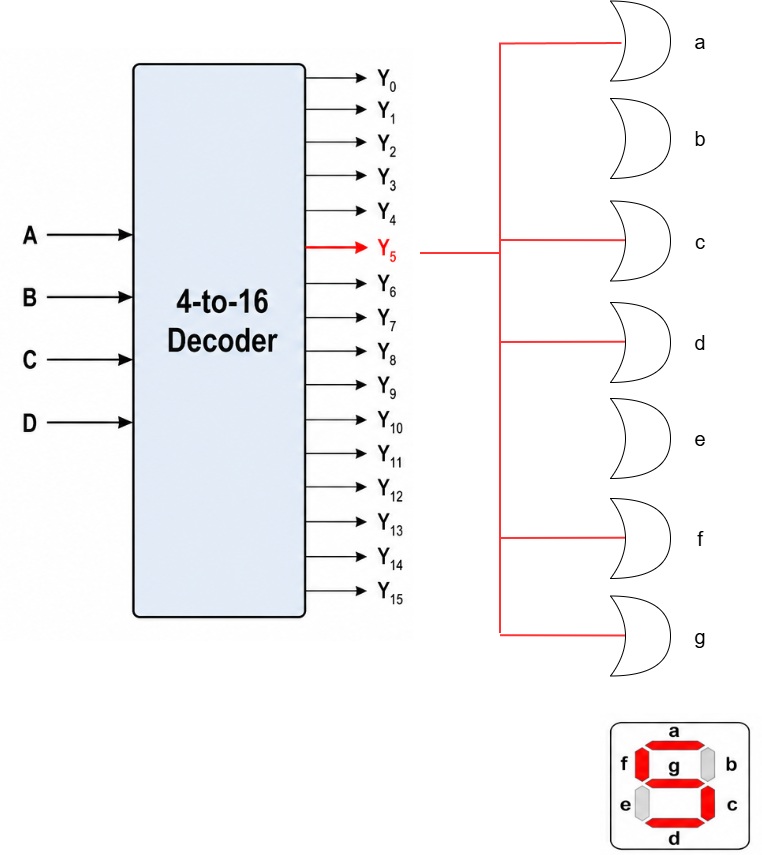
\includegraphics[width=0.50\textwidth]{4-16_led7.png}}{\fbox{\parbox[c][0.56\textwidth][c]{0.50\textwidth}{\centering Figure source unavailable in standalone preview}}}
    \caption{Illustrative $Y_5$ routes for displaying digit 5 (not the complete routing matrix).}
    \label{fig:decoder_or_topo}
\end{figure}

% --- MỤC IV: TRIỂN KHAI VÀ KẾT QUẢ THỰC NGHIỆM ---
\section{Implementation and Experimental Results}
\subsection{Experimental Setup}
The five primary designs were checked as complete small combinational functions, while the 8-bit comparator and PLA cases probe scale and external input data. Table~\ref{tab:benchmarks} distinguishes decoder states from actual routed connections: the latter sum the lengths of all output ON-sets and may exceed $2^n$ because outputs share minterms. It also makes clear why a 3-bit comparator has six physical input wires. The tests run on generated routing and RTL; they do not constitute fabrication or post-layout characterization.

\begin{table}[t]
\caption{Primary benchmark structure; connections count $Y_j$ references across all outputs.}
\label{tab:benchmarks}
\centering\small
\begin{tabular}{lrrrr}
\toprule
Circuit & Inputs & Outputs & Decoder states & Connections \\
\midrule
Half adder & 2 & 2 & 4 & 3 \\
Full adder & 3 & 2 & 8 & 8 \\
2-to-1 MUX & 3 & 1 & 8 & 4 \\
BCD to 7-segment & 4 & 7 & 16 & 49 \\
3-bit comparator & 6 & 3 & 64 & 64 \\
\bottomrule
\end{tabular}
\end{table}

\subsection{Functional and Parser Validation}
The five minterm benchmarks---half adder, full adder, 2-to-1 multiplexer, BCD display, and 3-bit comparator---span 2--6 inputs and 1--7 outputs \cite{benchmark_dataset}. The oracle enumerated 4, 8, 8, 16, and 64 input states (100 total), comparing the 94 states with specified outputs and skipping six BCD don't-cares. The BCD implementation's zero outputs on those six states were also checked as a deterministic behavior of this RTL, but zero was not required by the partially specified BCD function.

To test whether the oracle can detect defects, 78 deliberate dataset/routing mutations were injected. The campaign included removing or adding an ON-set entry, replacing a valid entry, swapping output maps, clearing an output, duplicating a routed pin, and using an out-of-range pin. All 78 were detected in this campaign; the count is a mutation score for these operators and benchmarks, not a universal guarantee of oracle correctness. Parser tests independently reject malformed JSON, missing fields, duplicate or unknown pins, inconsistent decoder dimensions, and explicit active-low requests. No unsupported mode is silently compiled as active-high OR logic.

\subsection{Scalability and External Benchmarks}
The 8-bit magnitude comparator compares two 8-bit operands, uses 16 input wires and a 16-to-65,536 decoder, and passed exhaustive equivalence over its 65,536 input combinations. Table~\ref{tab:scale} reports recorded generation/validation/RTL-flow measurements rather than extrapolated hardware performance. A separate synthetic series expands explicit minterm sets up to $n=20$. At $n=21$, a configured $2^{20}$-state safety bound rejects the case before generation; this is not an observed operating-system out-of-memory failure. The 8-bit comparator and generic $n=16$ have the same decoder width but different ON-set densities and JSON sizes, so input count alone is not a sufficient cost predictor.

\begin{table}[t]
\caption{Selected recorded software-scale results. MB denotes $10^6$ bytes for the JSON file.}
\label{tab:scale}
\centering\small
\begin{tabular}{lrrrr}
\toprule
Case & Input wires & States & JSON size (MB) & Flow time (s) \\
\midrule
8-bit comparator & 16 & 65,536 & 1.10 & 4.87 \\
Generic $n=16$ & 16 & 65,536 & 1.48 & 5.88 \\
Generic $n=20$ & 20 & 1,048,576 & 25.16 & 101.29 \\
Generic $n=21$ & 21 & 2,097,152 & -- & rejected \\
\bottomrule
\end{tabular}
\end{table}

Of 14 selected multi-output MCNC/LGSynth91 PLA benchmarks from an IWLS93 archive, 11 passed equivalence checks after expansion to explicit minterms. Three (22-, 23-, and 65-input cases) exceeded the configured single-decoder capacity bound and were not synthesized; they are not logic-verification failures. PLA conversion is an experimental preprocessing step, not a supported Boolean-expression/truth-table input mode of the user-facing front end. These cases expose both data-driven reuse and the poor scalability of a monolithic $2^n$ decoder.

\subsection{RTL Checks and BCD Don't-Cares}
Yosys synthesis and Icarus simulation completed for the five primary benchmarks and the 8-bit comparator; the simulations reported no mismatched vectors. Verilator lint reported no fatal errors, width warnings, undriven nets, or multidriven nets, but did report unused decoder bits and/or filename--module-name warnings. The RTL therefore passed these checks but is not warning-free, and physical design-rule checking was not performed.

For BCD, states 10--15 are absent from all segment ON-sets, so the generated RTL drives the segment outputs low for those inputs; $Y_{10}$--$Y_{15}$ are unused, not floating. The conventional don't-care baseline may assign arbitrary outputs there. In the saved mapping comparison, Decoder--OR and conventional logic had equal Sky130 area (116.36\,$\mu\mathrm{m}^2$ each), while Nangate45 areas were 23.67 and 25.00\,$\mu\mathrm{m}^2$, respectively. This isolated result does not establish a general area saving from don't-cares or a fair superiority claim when the invalid-state output contracts differ.

\subsection{Data Availability Statement}
The original dataset and verifier are available at \url{https://github.com/DepBo/Dataset_Paper_DecoderOr}. A separate repository for the revised manuscript, two-stage compiler, tests, experiment scripts, and results has been created at \url{https://github.com/DepBo/Decoder_OR_English}. At the time of this revision, its source upload is pending; until that upload is complete, the expanded results cannot be independently reproduced from the new repository alone.

% --- MỤC V: THẢO LUẬN ---
\section{Discussion}
\subsection{Hardware Boundary Analysis and Fan-in Limits}
Segment $c$ requires nine decoder pins, so the default $k=4$ compiler emits two RTL OR levels rather than one nine-operand expression. Functional equivalence and the fan-in bound were tested. For controlled 64- and 256-input OR reductions, a balanced tree reduced RTL depth from 63 to 3 and 255 to 4 relative to a linear chain. After Yosys/ABC mapping, however, each pair had the same cell count and critical-path stage count. Liberty-based delays were also equal: 492.70/232.35\,ps (Sky130 HD/Nangate45) at 64 inputs and 1014.42/237.97\,ps at 256 inputs. Thus, bounded RTL fan-in is validated, but a post-synthesis speedup is not. These are isolated reductions, not complete-benchmark or post-layout timing comparisons.

\subsection{Decoder Fan-out Limits}
When several outputs share $Y_i$, its capacitive load can increase transition time, not necessarily reduce steady-state logic voltage. In a controlled simplified 130\,nm SPICE model, the unbuffered average propagation delay increased from 25.28\,ps at one load to 350.52\,ps at 32 loads. At 64 loads the signal did not complete its low transition within the applied pulse; the reported 510.03\,ps average from that run should therefore not be treated as a fully settled cycle delay. These values come from a simplified transistor model and isolated test circuit, not a characterized post-layout benchmark.

Separately, Sky130 Yosys/ABC synthesis inserted buffers for the controlled loads in Table~\ref{tab:fanout}. The last column counts sinks driven by the output of each mapped buffer, read from the netlist, rather than estimating fan-out by dividing the original load count by $B+1$. ABC may also resize or restructure gates; these isolated loads do not prove that a particular benchmark decoder output was buffered.

\begin{table}[t]
\caption{Controlled mapped fan-out experiment; $B$ is the inserted-buffer count.}
\label{tab:fanout}
\centering\small
\begin{tabular}{rrrr}
\toprule
Load sinks & $B$ & Maximum buffer-output sinks & Buffered area overhead \\
\midrule
16 & 2 & 10 & 32.67\% \\
32 & 6 & 10 & 39.09\% \\
64 & 14 & 10 & 29.05\% \\
\bottomrule
\end{tabular}
\end{table}

The Python compiler does not insert buffers. Checks of maximum signal transition and load capacitance with OpenSTA were not completed. Neither were placement, detailed routing, parasitic extraction, or DRC. Thus, no electrical-limit or physical-design-rule compliance claim is made. Buffer selection is left to a technology-aware downstream tool, while reporting loads on complete generated benchmarks remains future work.

\subsection{System Generality: Survey on Arithmetic Circuit (Full Adder)}
For a 1-bit full adder, $Sum=\sum m(1,2,4,7)$ and $C_{out}=\sum m(3,5,6,7)$. Selecting this benchmark produces a 3-to-8 routing JSON; the same OR-tree compiler emits RTL without source-code changes. This shows data-driven reuse across two functions within the supported active-high architecture, not practical superiority for arbitrary circuits.

\subsection{Scalability to Complex Architectures}
The representation applies to other explicit minterm sets, including multiplexers and comparator outputs, but decoder width grows as $2^n$. The 8-bit and PLA results demonstrate both successful cases and the configured capacity limit; hierarchical partitioning or logic minimization is future work for much larger inputs.

\subsection{Study Limitations and Future Work}
The present implementation supports explicit minterm lists, MSB-first ordering, active-high decoder outputs, and OR/SOP output logic. It does not parse general Boolean expressions or user-supplied truth tables. Nor does the validator's ability to reject \texttt{Active\_Low}, \texttt{NAND}, or \texttt{POS} mean that these modes can be compiled. Extending them would require an unambiguous input format and polarity/operator fields, corresponding decoder and gate-generation rules, and new equivalence tests; this is planned work rather than a demonstrated feature.

The bounded-fan-in tree is a verified RTL construction, but the controlled synthesis comparison found no mapped timing gain. Future evaluation should compare flat and tree RTL on complete benchmarks under the same libraries and constraints, then use physical placement, routing, and extracted parasitics before making timing or congestion claims. Similarly, the fan-out test demonstrates that a downstream mapper can insert buffers in one setup, not that the Python compiler handles electrical violations. Library-specific transition/capacitance checks and full benchmark netlist audits are needed to establish that distinction.

Finally, a single explicit decoder grows exponentially, so the 8-bit comparator is a feasibility demonstration rather than evidence of unlimited scalability. Hierarchical decomposition, shared logic, or conventional minimization should be compared against the monolithic representation on more diverse functions. Verification is currently exhaustive only where the state space is tractable, and its 78 mutation results cover a defined fault set; larger randomized and formal-equivalence campaigns would improve confidence. The extended compiler and experimental scripts should also be released with versioned commands and library information so third parties can reproduce the new measurements.

% --- MỤC VI: KẾT LUẬN ---
\section{Conclusion}
The evaluated workflow converts explicit minterm lists into validated Decoder--OR routing JSON and bounded-fan-in Verilog. Functional, mutation, parser, synthesis, simulation, and selected external-benchmark checks support this result. The architecture remains limited to active-high sum-of-minterms logic; exponential decoder growth, absent post-layout checks, and the lack of measured timing or general area advantage limit its practical claims. Future work includes other input forms and gate polarities, hierarchical decomposition, and physical validation.

% --- DANH MỤC TÀI LIỆU THAM KHẢO ---
\begin{thebibliography}{00}

\bibitem{b1}
A. Costamagna and G. De Micheli, ``Accuracy recovery: A decomposition procedure for the synthesis of partially-specified Boolean functions,'' \emph{INTEGRATION, the VLSI journal}, vol. 78, pp. 112--125, 2023.

\bibitem{b2}
D. Balobas and N. Konofaos, ``Optimization of CMOS Decoders Using Three-Transistor Logic,'' \emph{MDPI Electronics}, vol. 14, no. 5, p. 914, 2025.

\bibitem{b3}
T. A. Ikwunne and S. O. Okide, ``Interactive Algorithms for the Verification of the Equality between Complex and Simplified Boolean-Algebra Expressions in Digital Decoders,'' \emph{Review of Computer Engineering Research}, vol. 7, no. 2, pp. 45--58, 2020.

\bibitem{benchmark_dataset}
P. L. N. Minh, P. T. Dung, T. M. Nhut, and L. N. H. Loc, ``Benchmark Dataset and Verification Testbench for Automated Decoder-OR Logic Synthesis,'' 2026. [Online]. Available: \url{https://github.com/DepBo/Dataset_Paper_DecoderOr.git}

\end{thebibliography}

\end{document}
